% !TEX encoding = UTF-8 Unicode
%\documentclass{beamer} %voce pode usar este modelo tambem
\documentclass{beamer}%[handout]{beamer}

% for XeLaTex use this code below
\usepackage{fontspec}
% \setmainfont[
%   Ligatures=TeX,
%   Extension=.otf,
%   BoldFont=cmunbx,
%   ItalicFont=cmunti,
%   BoldItalicFont=cmunbi,
% ]{cmunrm}
% \setsansfont[
%   Ligatures=TeX,
%   Extension=.otf,
%   BoldFont=cmunsx,
%   ItalicFont=cmunsi,
% ]{cmunss}


%\setmainfont{Roboto}
%\setsansfont[Scale=MatchUppercase]{Roboto Light}
%\setmonofont[Scale=MatchUppercase]{Hack}
\usepackage{xfrac,unicode-math}
%\setmathfont{Noto Serif}

% for LuaLatex use this code below for russian language
%\usepackage{fontspec}
%\setmainfont{CMU Serif}[Ligatures=TeX]
%\setsansfont{CMU Sans Serif}[Ligatures=TeX]

\usepackage{inputenc}
%\usepackage[utf8x]{inputenc}         % кодовая страница документа
\usepackage{indentfirst}   % русский стиль: отступ первого абзаца раздела
%\usepackage[utf8]{inputenc}
\usepackage[english]{babel}
\usepackage{graphicx,url, lastpage}
\usepackage{wrapfig}
\usepackage{ulem} %зачеркнуть


%%% Работа с таблицами
\usepackage{array,tabularx,tabulary,booktabs} % Дополнительная работа с таблицами
\usepackage{longtable}  % Длинные таблицы
\usepackage{multirow} % Слияние строк в таблице
\usepackage{makecell} % Перенос в таблице



\batchmode
% \usepackage{pgfpages}
% \pgfpagesuselayout{4 on 1}[letterpaper,landscape,border shrink=5mm]
\usepackage{amsmath,amssymb,enumerate,epsfig,bbm,calc,color,ifthen,capt-of}
%\usetheme{Berlin}
\usetheme{Berlin}
% skips the subsection headlines
\setbeamertemplate{headline}
{%
  \begin{beamercolorbox}[colsep=1.5pt]{upper separation line head}
  \end{beamercolorbox}
  \begin{beamercolorbox}{section in head/foot}
    \vskip2pt\insertnavigation{\paperwidth}\vskip2pt
  \end{beamercolorbox}%
  \begin{beamercolorbox}[colsep=1.5pt]{lower separation line head}
  \end{beamercolorbox}
}
% removes footline
\setbeamertemplate{footline}{}
% insert page number
\addtobeamertemplate{navigation symbols}{}{%
  \usebeamerfont{footline}%
  \usebeamercolor[fg]{footline}%
  \hspace{2em}%
  %\insertframenumber/\inserttotalframenumber
  \raisebox{1.3pt}[0pt][0pt]{\insertframenumber/\inserttotalframenumber}
}
\usepackage{enumitem}
%
%\setitemize{label=\usebeamerfont*{itemize item}%
%  \usebeamercolor[fg]{itemize item}
%  \usebeamertemplate{itemize item}}

\setlist[itemize]{%
  label=\usebeamerfont*{itemize item}%
  \usebeamercolor[fg]{itemize item}%
  \usebeamertemplate{itemize item}%
}%http://tex.stackexchange.com/a/24491
\setlist[enumerate,1]{%
  label=\protect\usebeamerfont{enumerate item}%
  \protect\usebeamercolor[fg]{enumerate item}%
  \insertenumlabel.%
}
% definition of new key for enumitem:
\makeatletter
\enitkv@key{enumitem}{overlay}{%
  \beamerdefaultoverlayspecification{#1}%
}
\makeatother
%\setbeamerfont{title}{shape=\itshape,family=\rmfamily}
%\setbeamerfont{alerted text}{shape=\itshape,family=\rmfamily}
%\setbeamerfont{palette primary}{shape=\itshape,family=\rmfamily}
%\setbeamerfont{palette secondary}{shape=\itshape,family=\rmfamily}
%\setbeamerfont{palette tertiary}{shape=\itshape,family=\rmfamily}
%\setbeamerfont{palette quaternary}{shape=\itshape,family=\rmfamily}
%\setbeamerfont{headline}{shape=\itshape,family=\rmfamily, size=\tiny}
%\setbeamerfont{headline}{size*={6pt}}

%\usecolortheme{senac}



\newcommand{\N}{\mathbb{N}}
\newcommand{\Z}{\mathbb{Z}}
\newcommand{\R}{\mathbb{R}}




% Multiple columns
\usepackage{multicol}



%listings for code

\usepackage{color} %% это для отображения цвета в коде
\usepackage{listings} %% собственно, это и есть пакет listings

\usepackage{caption}
\DeclareCaptionFont{white}{\color{black}} %% это сделает текст заголовка белым white
% black, blue, brown, cyan, darkgray, gray, green, lightgray, lime, magenta, olive, orange, pink, purple, red, teal, violet, white, yellow
%% код ниже нарисует серую рамочку вокруг заголовка кода.
\definecolor{light-gray}{gray}{0.9}
\DeclareCaptionFormat{listing}{\colorbox{light-gray}{\parbox{\textwidth}{#1#2#3}}}
\captionsetup[lstlisting]{format=listing,labelfont=white,textfont=white}


\lstset{ %
  language=Java,                 % выбор языка для подсветки (здесь это С)
  basicstyle=\small\sffamily, % размер и начертание шрифта для подсветки кода
  morekeywords={class},
  numbers=left,               % где поставить нумерацию строк (слева\справа)
  numberstyle=\tiny,           % размер шрифта для номеров строк
  stepnumber=1,                   % размер шага между двумя номерами строк
  numbersep=5pt,                % как далеко отстоят номера строк от подсвечиваемого кода
  backgroundcolor=\color{white}, % цвет фона подсветки - используем \usepackage{color}
  showspaces=false,            % показывать или нет пробелы специальными отступами
  showstringspaces=false,      % показывать или нет пробелы в строках
  showtabs=false,             % показывать или нет табуляцию в строках
  frame=single,              % рисовать рамку вокруг кода
  tabsize=2,                 % размер табуляции по умолчанию равен 2 пробелам
  captionpos=t,              % позиция заголовка вверху [t] или внизу [b]
  breaklines=true,           % автоматически переносить строки (да\нет)
  breakatwhitespace=false, % переносить строки только если есть пробел
  escapeinside={\%*}{*)}   % если нужно добавить комментарии в коде
}




% \textbf{Automated Testing System for Android Applications of Samsung Innovation Campus Learners}

% \textbf{Supervisor: Olga V. Maksimenkova, \\
% Associate Professor, \\ Faculty of Computer Science / School of Software Engineering}



%-------------------------Titulo/Autores/Orientador------------------------------------------------
\title[Developing an Android Application for Indoor Control Inspections of Construction Progress]{
  Developing an Android Application for Indoor Control Inspections of \\ Construction Progress}
%\date{Fuad Aleskerov,  Dmitry Egorov, Vyacheslav Yakuba \\ \ \\  Higher School of Economics \\ \ \\  May 23, 2022 }%\\ Moscow, 2022 }
\date{ Dmitry Egorov \\ \ \\   Supervisor \\ Aleksey D. Shadrikov \\ Senior Specialist \\ AI Track Curator at Samsung Innovation Campus  \\ \ \\
HSE University / 29 June 2024 }%\\ Moscow, 2022 }
\author[Dmitry Egorov \hspace{10em} \insertpagenumber \ /  \pageref{LastPage}]{        }

%-------------------------Logo na parte de baixo do slide------------------------------------------
%\pgfdeclareimage[height=0.7cm]{senac-logo}{senac-logo.pdf}
%\logo{\pgfuseimage{senac-logo}\hspace*{0.5cm}}


%----------------------------- Declare
%\pgfdeclareimage[height=2.7cm]{turnir}{togo7}


%-------------------------Este código faz o menuzinho bacana na parte superior do slide------------
% \AtBeginSection[]
% {
%   \begin{frame}<beamer>
%     \frametitle{Содержание}
%     \tableofcontents[currentsection]
%   \end{frame}
% }
% \beamerdefaultoverlayspecification{<+->}
% -----------------------------------------------------------------------------
\begin{document}
% -----------------------------------------------------------------------------

\newenvironment{changemargin}{%
\begin{list}{}{%
\setlength{\topsep}{0pt}%
\setlength{\leftmargin}{-0.4cm}%
\setlength{\rightmargin}{-0.4cm}%
\setlength{\listparindent}{\parindent}%
\setlength{\itemindent}{\parindent}%
\setlength{\parsep}{\parskip}%
}%
\item[]}{\end{list}}

%---Gerador de Sumário---------------------------------------------------------
\frame{\titlepage}
% \begin{frame}{Содержание}
%   \tableofcontents
%  \end{frame}
\setlist{nolistsep, itemsep=3pt,parsep=0pt,leftmargin=1pt}

%\logo{}

%-----------------------------------------------------------------------------
%\section[System overview]{System overview}
%\begin{frame}{Introduction}
%\footnotesize

%Mobile devices → {\usebeamercolor[fg]{structure} On-device inference }



%\begin{figure}[h]
%  \begin{minipage}[h]{0.4\linewidth}
%    \hbox{\hspace{-0.1em}\includegraphics[width=\linewidth]{img/three_stages_scheme.png}}
%    %\caption{\footnotesize Integration into existing infrastructure}
%  \end{minipage}
%\end{figure}



%\end{frame}
%------------------------------------------------------------------------------
%-----------------------------------------------------------------------------
\section[Introduction]{Introduction}
\begin{frame}{Introduction}
\footnotesize

We propose customisable approaches to the system specifically for Android labs

\begin{itemize}

\item Traditional methods of indoor control inspections face challenges due to manual processes and data delays

\item {\usebeamercolor[fg]{structure} Main goal}: to develop software that provides real-time inspections with on-device model inference

\item Advantages: improved accuracy, reduced time on-site, and instant data synchronization.

\item Prior research has explored construction progress monitoring using computer vision, AR, robotics, but with a focus on outdoor picture.

\end{itemize}

Objectives are:

1. Developing a client-server system architecture for communication and data transfer.

2. Implementing an Android application with adapted interface and inspection features (object recognition).

3. Integrating efficient on-device object recognition models and implementing additional post-processing tasks.

4. Evaluating the system under several mocks.



\end{frame}
%---------------------------------------------------------------------------
%------------------------------------------------------------------------------
\begin{frame}{Methodology}
\begin{changemargin}
\footnotesize


%{\usebeamercolor[fg]{structure} quantitative (with mathematical models)}  / qualitative (expert-based)

 \begin{figure}[h]
  \begin{minipage}[h]{0.65\linewidth}
  \hbox{\hspace{-0.1em}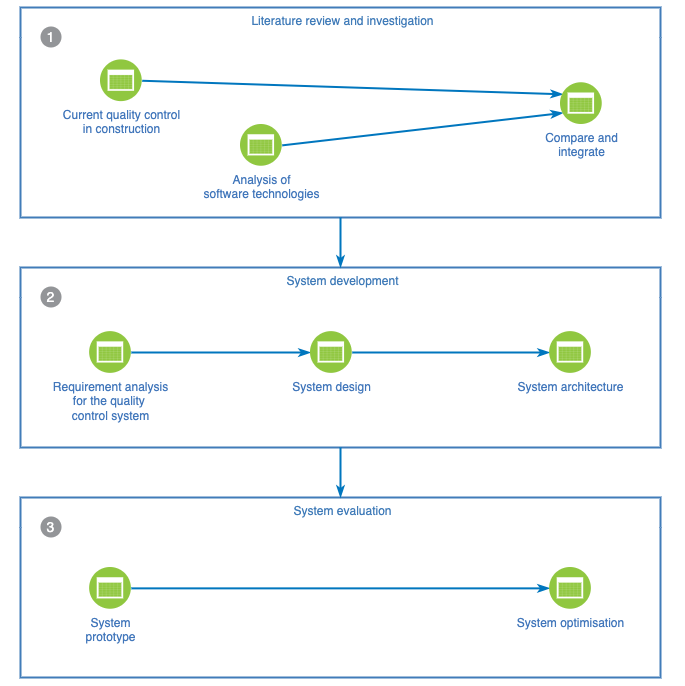
\includegraphics[width=\linewidth]{img/stages_of_research}}
  \end{minipage}
  \end{figure}


\end{changemargin}
\end{frame}
%------------------------------------------------------------------------------
%------------------------------------------------------------------------------
\section[System overview]{System overview}
\begin{frame}{High-level system architecture overview with data flows}
\begin{changemargin}
\footnotesize

\begin{figure}[h]
\begin{minipage}[h]{\linewidth}
\hbox{\hspace{-0.8em}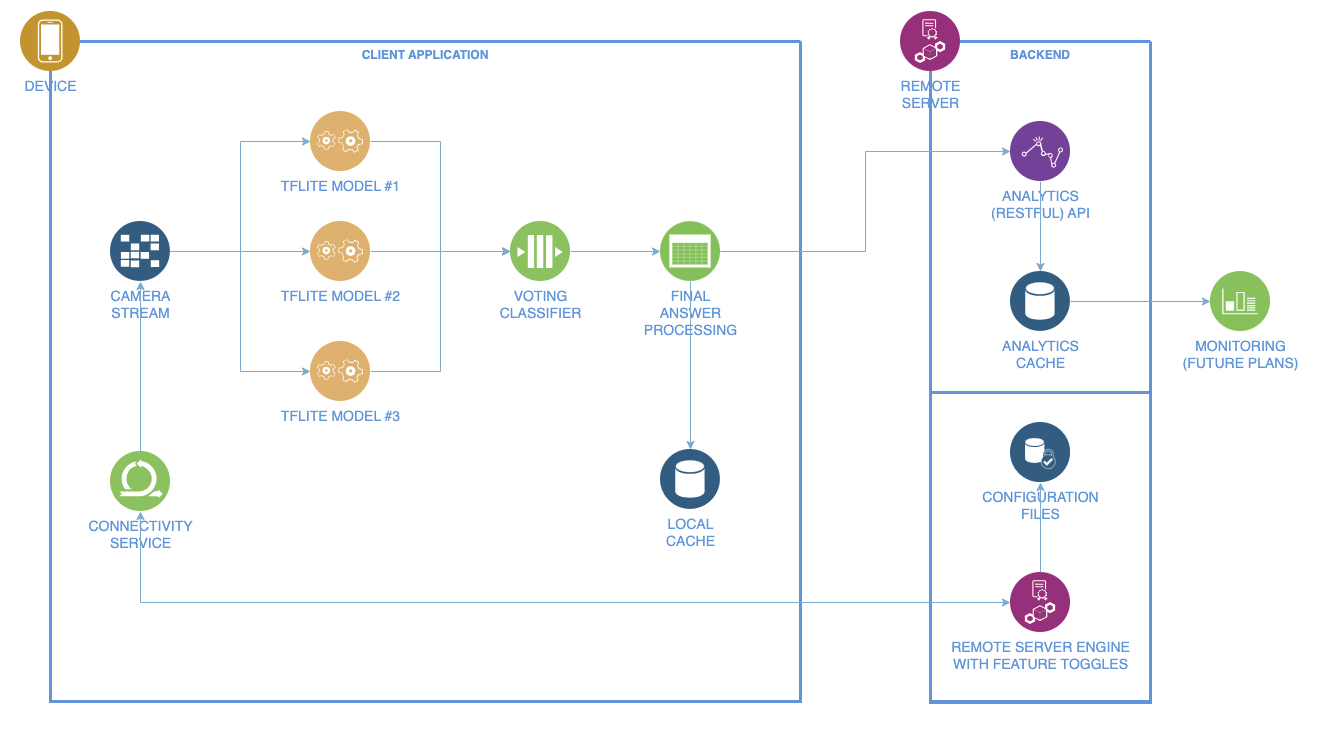
\includegraphics[width=1.08\linewidth]{img/system_overview}}
\end{minipage}
\end{figure}



\end{changemargin}
\end{frame}
%------------------------------------------------------------------------------
%-----------------------------------------------------------------------------
\begin{frame}{On-device \textit{vs} server-based inference comparison}
\footnotesize


\begin{table}[h!]
%\caption{Comparison of our solution with server-based inference and conventional approaches}
\centering\begin{tabulary}{1.03\textwidth}{LLLL}
\toprule
\textbf{Aspect}  & \textbf{Our Solution (On-Device Inference)}   & \textbf{Server-Based Inference}  & \textbf{Conventional Approaches}    \\
\midrule
Recognition  & Automated via on-device ML model   & Automated via ML model on server & Manual inspection and identification \\
Latency             & Low                                & Moderate                         & High                                 \\
Offline Capability  & Fully functional                   & Not available                    & Fully functional (manual processes)  \\
Model Update        & Requires model sync                & Easy to update                   & Not applicable                       \\
Inspection Accuracy & High with antifraud module         & High with antifraud module       & Variable                             \\
Report Generation   & Automated report generation        & Automated report generation      & Manual report preparation            \\
\bottomrule
\end{tabulary}
\label{table:solution_comparison}
\end{table}




\end{frame}
%---------------------------------------------------------------------------
%------------------------------------------------------------------------------
\begin{frame}{Soft Voting Classifier}
\begin{changemargin}
\footnotesize

\begin{figure}[h]
\begin{minipage}[h]{0.91\linewidth}
\hbox{\hspace{-2em}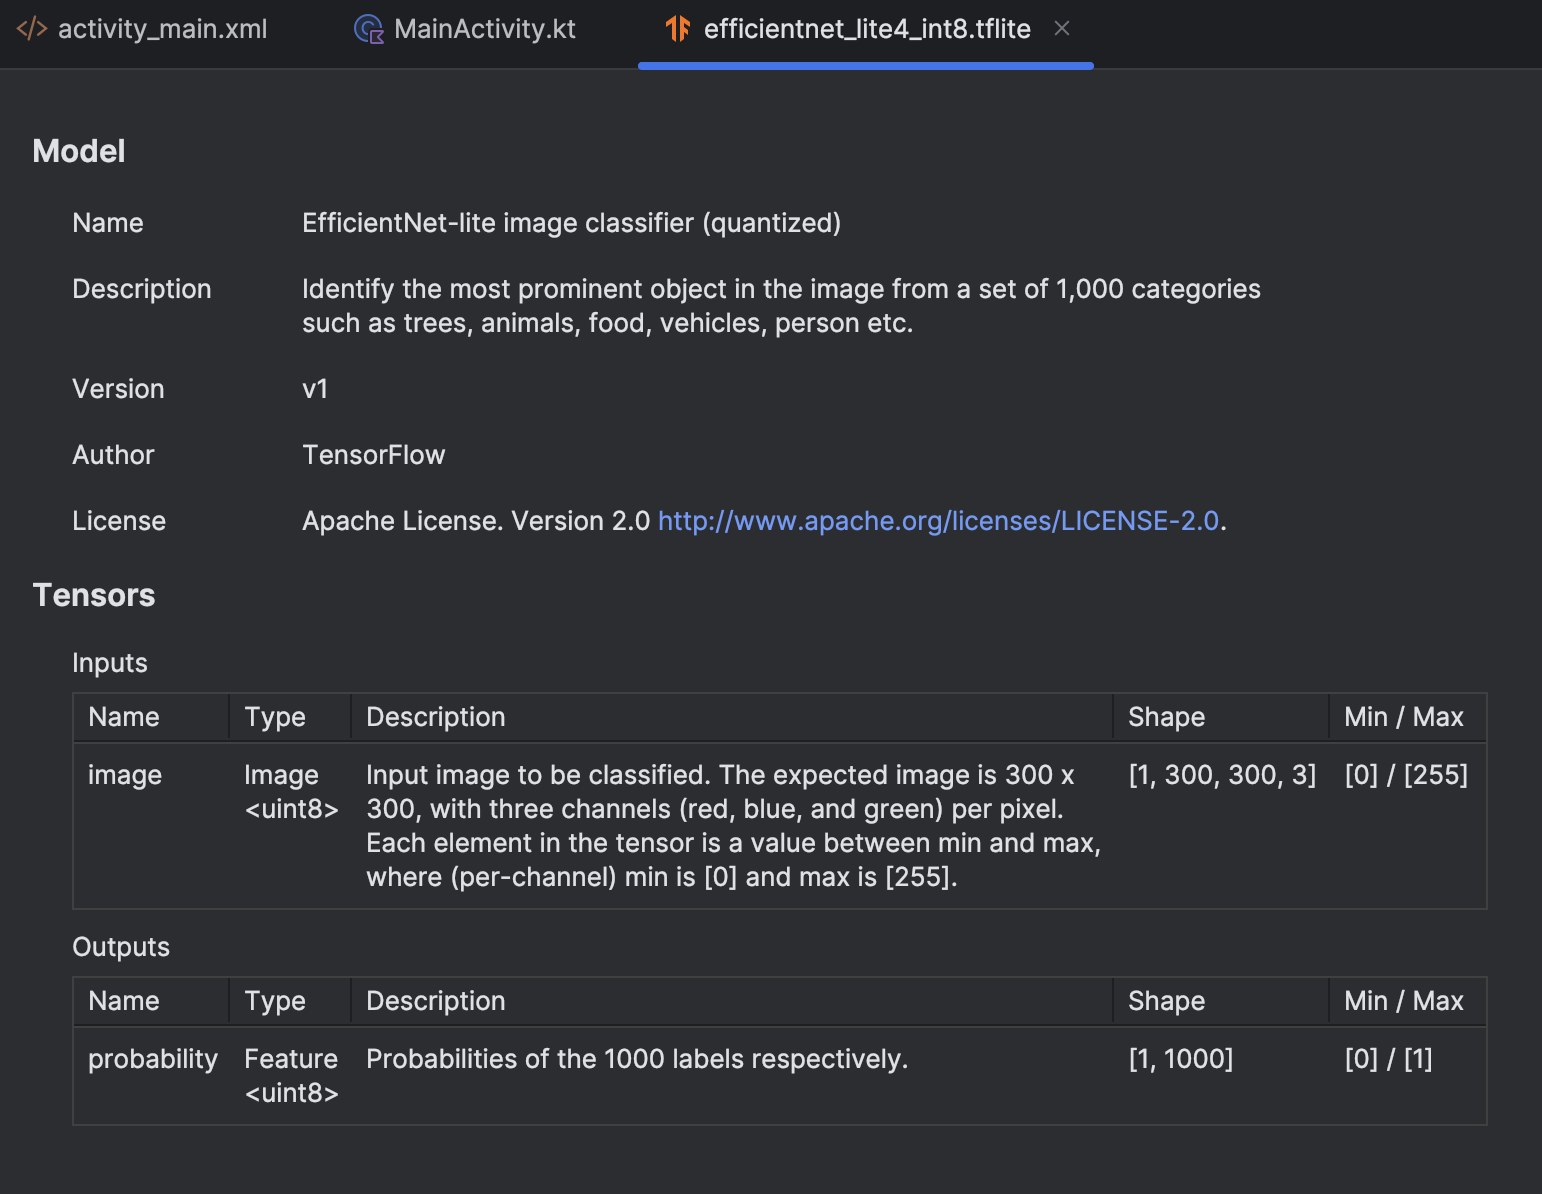
\includegraphics[width=0.91\linewidth]{img/efficientnet_spec}}
\end{minipage}
\end{figure}

\end{changemargin}
\end{frame}
%------------------------------------------------------------------------------
%------------------------------------------------------------------------------
\begin{frame}{Android Application Development}
\begin{changemargin}
\footnotesize

\begin{table}[h]
\caption{List of frameworks for the app}
\centering\begin{tabular}{rl}
\toprule
Library   & Description                          \\
\midrule
CameraX  & Interacting with the camera and showing preview \\
NavigationKTX   & Navigating inside the app and switching between fragments                   \\
DataStore       & Saving data locally                   \\
TFLite       & Image classification models inference \\ & MobileNet v3, EfficientNet-Lite4, and DenseNet                  \\
Diskord     & Connecting to Discord server via REST  \\
JUnit       & Launching unit-tests for the View Model (MVVM architecture)                \\
\bottomrule
\end{tabular}
\label{table:libraries}
\end{table}

\vspace{1.5ex} Server for retrieving the necessary configuration settings and feature flags, see FeatureService Kotlin class

Sealed class (with descendants such as window, door and radiator) for abstract object that we detect

pre-trained on ImageNet--1K (ILSVRC-2012-CLS dataset)

\end{changemargin}
\end{frame}
%------------------------------------------------------------------------------
%------------------------------------------------------------------------------
\begin{frame}{Degree of credibility}
\begin{changemargin}
\footnotesize

Modern mobile devices are equipped with a variety of sensors that can provide some information about the device's environment
\begin{itemize}
    \item GPS sensor
    \item Accelerometer
    \item Gyroscope
    \item Magnetic field sensor
    \item Proximity sensor
\end{itemize}

 For example, the GPS location does not match the expected construction site coordinates → a warning is triggered
 
\end{changemargin}
\end{frame}
%------------------------------------------------------------------------------
%------------------------------------------------------------------------------
\begin{frame}{UI}
\begin{changemargin}
\footnotesize


\begin{figure}[h]
\begin{minipage}[h]{0.3\linewidth}
\hbox{\hspace{-2em}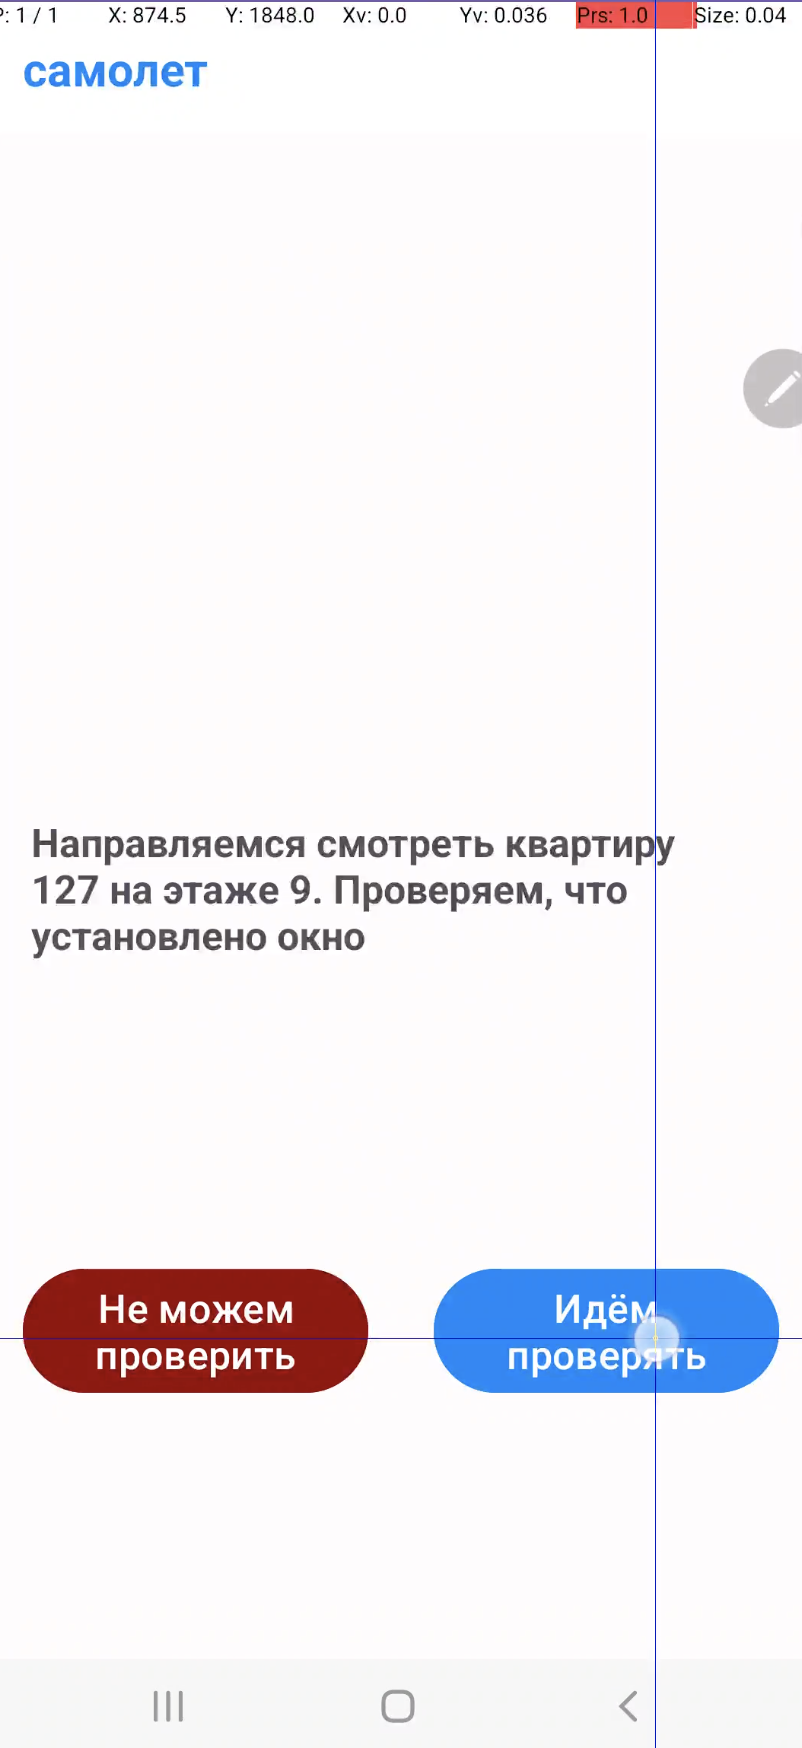
\includegraphics[width=\linewidth]{img/app_ui}}
\end{minipage}
\end{figure}

\end{changemargin}
\end{frame}
%------------------------------------------------------------------------------
%------------------------------------------------------------------------------
\section[Results]{Results}
\begin{frame}{Results and Discussion}
\begin{changemargin}
\footnotesize
%\scriptsize

\begin{itemize}
\item<1-> Our comprehensive solution for for indoor control inspections of construction progress
\item<1-> A server mock and a client application
\item<1-> On-device ML for real-time inference directly on the Android phone or tablet
\item<1-> The minimum supported version is Android Oreo (API 26)
\item<1-> The ML system is implemented using TensorFlow Lite, employing lightweight models optimised for on-device inference
\item<1-> Standard indoor lighting conditions, though variations in lighting are common in actual construction sites
\item<1-> The application requires Internet connectivity, at least during app launch
\end{itemize}

\vspace{1.5ex} Our work contributes to the field by providing a practical solution for construction progress monitoring and highlights improvements over existing methods in terms of credibility and data transfer delays \vspace{1.2ex}

Future directions for the Android part: extend support for compose layouts

\vspace{1.10ex} Code Availability Statement. https://github.com/DmitrijEgorow/AndroidFramingScanner




\end{changemargin}
\end{frame}
%------------------------------------------------------------------------------
%------------------------------------------------------------------------------
\section[References]{References}
\begin{frame}{ }
\begin{changemargin}
\footnotesize

\begin{minipage}[t][0.8715\textheight]{\linewidth}
\begin{center}
Thank you! \vspace{1.5ex}
\end{center}

\scriptsize
\begin{enumerate}

\item<1->[[1\text{]}] Y. Zou, A. Kiviniemi, and S. W. Jones, “A review of risk management through BIM and BIM-related technologies”, Safety science, vol. 97, pp. 88–98, 2017.
\item<1->[[2\text{]}] X. Wang, P. E. Love, M. J. Kim, C.-S. Park, C.-P. Sing, and L. Hou, “A conceptual framework for integrating building information modeling with augmented reality”, Automation in construction, vol. 34, pp. 37–44, 2013.
\item<1->[[3\text{]}] J. Wang, W. Sun, W. Shou, X. Wang, C. Wu, H.-Y. Chong, Y. Liu, and C. Sun, “Integrating BIM and LiDAR for real-time construction quality control”, Journal
of Intelligent & Robotic Systems, vol. 79, pp. 417–432, 2015.
\item<1->[[4\text{]}] M. Golparvar-Fard, F. Pena-Mora, and S. Savarese, “Automated progress monitoring using unordered daily construction photographs and IFC-based building information models”, Journal of Computing in Civil Engineering, vol. 29, no. 1, p. 04 014 025, 2015.
\item<1->[[5\text{]}] S. Halder, K. Afsari, J. Serdakowski, S. DeVito, M. Ensafi, and W. Thabet, “Real- time and remote construction progress monitoring with a quadruped robot using augmented reality”, Buildings, vol. 12, no. 11, p. 2027, 2022.
\item<1->[[6\text{]}] C. Zhang and D. Arditi, “Automated progress control using laser scanning technology”, Automation in construction, vol. 36, pp. 108–116, 2013.
\item<1->[[7\text{]}] M. Golparvar-Fard, F. Peña-Mora, and S. Savarese, “Integrated sequential as-built and as-planned representation with d 4 ar tools in support of decision-making tasks in the aec/fm industry”, Journal of Construction Engineering and Management, vol. 137, no. 12, pp. 1099–1116, 2011.



\end{enumerate}


\vspace{3ex}% or \vfill
% Dmitry Egorov, tegorkrsk@gmail.com
\end{minipage}


%\vspace{20ex}

\end{changemargin}
\end{frame}
%------------------------------------------------------------------------------
%------------------------------------------------------------------------------

\begin{frame}{ }
\footnotesize

\begin{minipage}[t][0.8715\textheight]{\linewidth}
\begin{center}
Thank you! \vspace{1.5ex}
\end{center}

\scriptsize
\begin{enumerate}

\item<1->[[8\text{]}] M. Foroughi Sabzevar, M. Gheisari, and J. Lo, “Development and assessment of a sensor-based orientation and positioning approach for decreasing variation in camera viewpoints and image transformations at construction sites”, Applied Sciences, vol. 10, no. 7, p. 2305, 2020.
\item<1->[[9\text{]}] S. Zollmann, C. Hoppe, S. Kluckner, C. Poglitsch, H. Bischof, and G. Reitmayr, “Augmented reality for construction site monitoring and documentation”,
Proceedings of the IEEE, vol. 102, no. 2, pp. 137–154, 2014.
\item<1->[[10\text{]}] Y. Zhou, H. Luo, and Y. Yang, “Implementation of augmented reality for segment displacement inspection during tunneling construction”, Automation in Construction, vol. 82, pp. 112–121, 2017.
\item<1->[[11\text{]}] C.-S. Park, D.-Y. Lee, O.-S. Kwon, and X. Wang, “A framework for proactive construction defect management using BIM, augmented reality and ontology-based data collection template”, Automation in construction, vol. 33, pp. 61–71, 2013.
\item<1->[[12\text{]}] A. Howard, M. Sandler, G. Chu, L.-C. Chen, B. Chen, M. Tan, W. Wang, Y. Zhu, R. Pang, V. Vasudevan, et al., “Searching for mobilenetv3”, in Proceedings of the IEEE/CVF international conference on computer vision, 2019, pp. 1314–1324.
\item<1->[[13\text{]}] G. Huang, Z. Liu, L. van der Maaten, and K. Weinberger, “Densely connected convolutional networks”, arXiv preprint arXiv:1608.06993, 2016.
\item<1->[[14\text{]}] M. Tan and Q. Le, “Efficientnet: Rethinking model scaling for convolutional neural networks”, in International conference on machine learning, PMLR, 2019.


\end{enumerate}


\vspace{3ex}% or \vfill
% Dmitry Egorov, tegorkrsk@gmail.com
\end{minipage}


%\vspace{20ex}

\end{frame}
%------------------------------------------------------------------------------
%------------------------------------------------------------------------------
\begin{frame}{Soft Voting Classifier}
\begin{changemargin}
\footnotesize


\begin{figure}[h]
\begin{minipage}[h]{0.91\linewidth}
\hbox{\hspace{-2em}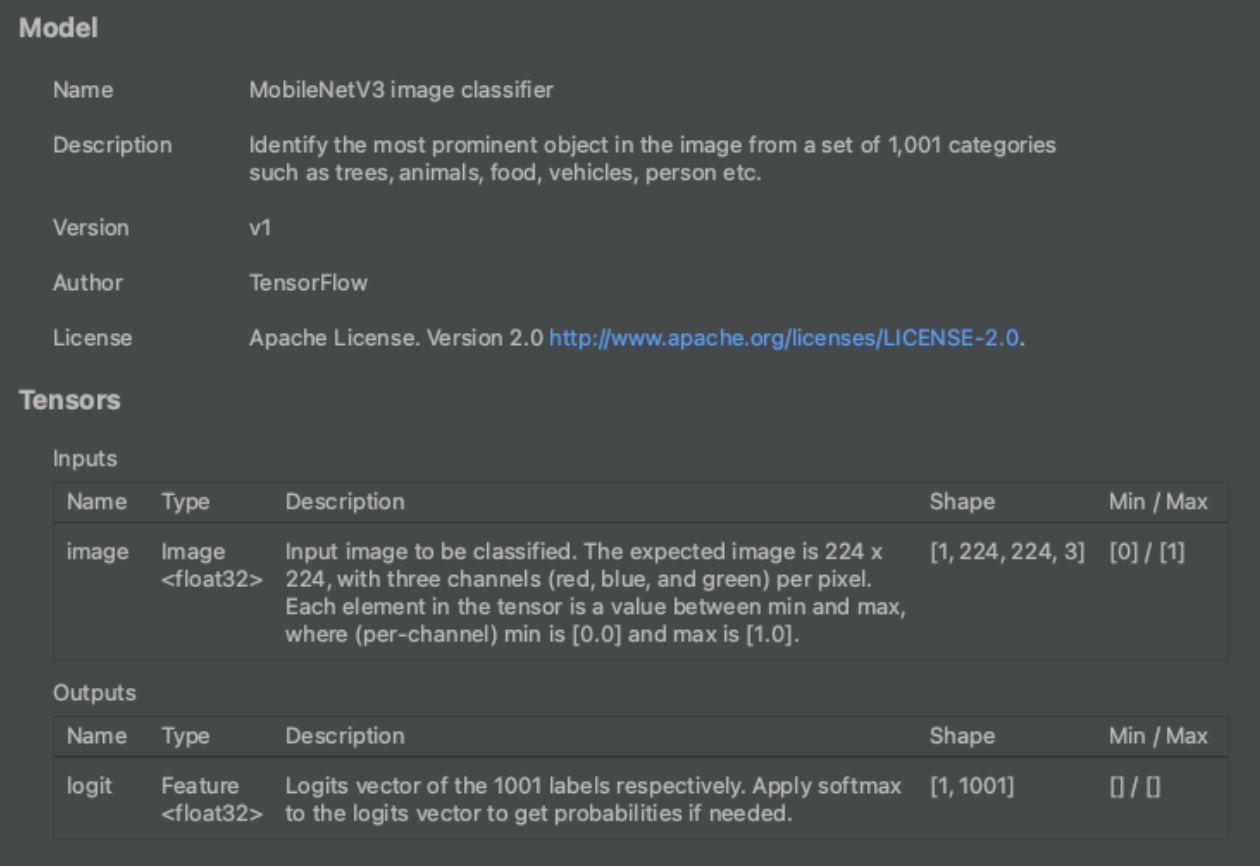
\includegraphics[width=\linewidth]{img/mobilenet_v3_spec}}
\end{minipage}
\end{figure}

\end{changemargin}
\end{frame}
%------------------------------------------------------------------------------

\end{document}
%-----------------------------------------------Este comentario nunca aparecera